\documentclass[11pt]{beamer}
\usepackage[UTF8,scheme=plain]{ctex}
\usepackage{listings}
\usepackage[utf8]{inputenc}
\usepackage[T1]{fontenc}
\usepackage{amsmath}
\usepackage{amsfonts}
\usepackage{amssymb}
\usepackage{mathrsfs}
\usepackage{graphicx}
\usetheme{Boadilla}

\usepackage{framed} % 可以用 \begin{shaded},即背景色块
\definecolor{shadecolor}{rgb}{0.9,0.9,0.9}

\newcommand{\kong}[1][0.5]{\vspace{#1cm}}

\begin{document}
	\author{ 路毅 \hspace{0.3cm} 曲阜师范大学 }
	\date{\number\year 年 \number\month 月 \number\day 日}
	\title{勒让德多项式 球函数}

\begin{frame}
	\maketitle
\end{frame}

\kaishu

\begin{frame}{勒让德多项式 球函数}
\begin{itemize}
	\item {\color{blue}第一节:斯图姆-刘维尔理论}
	\vspace{1cm}
	\item 第二节:勒让德多项式
	\vspace{1cm}
	\item 第三节:连带勒让德多项式
	\vspace{1cm}
	\item 第四节:球函数、球形区域上的狄利克雷问题
\end{itemize}
\end{frame}

\begin{frame}{斯图姆-刘维尔理论}

2阶常微分方程的一般形式为:区间$(a,b)$内,
\begin{equation}
L u(x) = p_0 (x) \frac{d^2}{dx^2} u + p_1(x) \frac{d}{dx} u + p_2 u,
\end{equation}
$p_0 (x)$在区间$(a,b)$内没有零点,但允许在$a,b$点为零点。

定义
\begin{equation}
\langle v | L | u \rangle = \int^b_a v ( p_0 u'' + p_1 u' + p_2 u ) dx,
\end{equation}
\end{frame}

\begin{frame}{自伴算子}
我们想知道,什么时候有
\begin{equation}
\langle v | L | u \rangle - \langle u | L | v \rangle = 0,
\end{equation}
于是我们计算
\begin{eqnarray}
\int^b_a vp_0 u'' dx &=& \int^b_a p_0 v du' = p_0 v u' |^b_a - \int^b_a u' (p_0 v)' dx \nonumber\\
&=& p_0 v u' |^b_a - \int^b_a p'_0 v u' dx - \int^b_a p_0 v' u' dx,
\end{eqnarray}
对称地,
\begin{equation}
\int^b_a u p_0 v'' dx = p_0 v'u |^b_a - \int^b_a p'_0 v'u dx - \int^b_a p_0 v'u' dx,
\end{equation}

\end{frame}

\begin{frame}{自伴算子}
所以有
\begin{equation}
\int^b_a v p_0 u'' dx - \int^b_a u p_0 v'' dx
= p_0 (vu' - uv')|^b_a - \int^b_a p'_0 (vu' - uv') dx,
\end{equation}
另外,
\begin{eqnarray}
\int^b_a p_1 v u' dx - \int^b_a p_1 u v' dx 
&=& \int^b_a p_1 (vu' - uv') dx. \\
\int^b_a p_2 vu dx - \int^b_a p_2 uv dx &=& 0.
\end{eqnarray}
所以有
\begin{equation}
\langle v | L | u \rangle - \langle u | L | v \rangle = p_0 (v'u - uv')|^b_a - \int^b_a (p'_0 - p_1)(v'u - uv') dx.
\end{equation}

\end{frame}

\begin{frame}{自伴算子}
\begin{equation}
\langle v | L | u \rangle - \langle u | L | v \rangle = p_0 (v'u - uv')|^b_a - \int^b_a (p'_0 - p_1)(v'u - uv') dx.
\end{equation}
所以,如果有
\begin{equation}
\left\{
\begin{aligned}
&& p_0 (vu' - uv') |^b_a = 0, \\
&& p'_0 - p_1 = 0, \forall x \in (a,b).
\end{aligned}
\right.
\end{equation}
则有$\langle v | L | u \rangle = \langle u | L | v \rangle$,则称$L$为自伴算子
\footnote{自伴算子推广到复数,就是量子力学中的厄米算符。}。

\end{frame}

\begin{frame}{自伴算子的本征方程}
广义的本征方程:在$(a,b)$上,
\begin{equation}
L u(x) + \lambda \omega(x) u(x) = 0,
\end{equation}
其中,$L$是一个自伴算子,$\lambda$称作本征值,$\omega(x)$称作权重函数(weighting function),$u(x)$称作本征函数。

\kong[0.5]
广义的内积
\begin{equation}
\langle v | u \rangle = \int^b_a v(x) \omega(x) u(x) dx.
\end{equation}
正交则定义为
\begin{equation}
\langle v | u \rangle = 0.
\end{equation}

\end{frame}

\begin{frame}{不同本征值对应的本征函数正交}

若有$ (\lambda_i, u_i)$以及$(\lambda_j, u_j)$,满足$\lambda_i \neq \lambda_j$,
\begin{eqnarray}
L u_i + \lambda_i \omega u_i &=& 0, \\
L u_j + \lambda_j \omega u_j &=& 0.
\end{eqnarray}
则有
\begin{equation}
\langle u_i | L | u_j \rangle = - \lambda_i \langle u_i | u_j \rangle = \langle u_j | L | u_i \rangle = - \lambda_j \langle u_j | u_i \rangle,
\end{equation}
所以有
\begin{equation}
\langle u_i | u_j \rangle = 0,
\end{equation}
即$u_i, u_j$正交。
\end{frame}

\begin{frame}{例:勒让德函数正交性}
勒让德微分方程为:$[-1,1]$上,
\begin{equation}
(1-x^2) u'' - 2x u' + n(n+1) u = 0, -1 \leq x \leq 1.
\end{equation}
即$p_0 (x) = 1-x^2, p_1(x) = -2x, p_2(x) = 0, \omega(x) = 1, \lambda = n(n+1)$。
所以自然有,$n\neq m$时,勒让德函数$P_n, P_m$的正交性
\begin{equation}
\langle P_n | P_m \rangle = \int^1_{-1} P_n(x) P_m(x) dx = 0.
\end{equation}

\end{frame}

\begin{frame}{勒让德多项式 球函数}
\begin{itemize}
	\item 第一节:斯图姆-刘维尔理论
	\vspace{1cm}
	\item {\color{blue}第二节:勒让德多项式}
	\vspace{1cm}
	\item 第三节:连带勒让德多项式
	\vspace{1cm}
	\item 第四节:球函数、球形区域上的狄利克雷问题
\end{itemize}
\end{frame}

\begin{frame}{勒让德函数}
复变函数
\begin{equation}
G(x,z) = \frac{1}{ \sqrt{1-2xz+z^2} },
\end{equation}
其中$z \in C, x \in R$且$|x| \leq 1$。
本节所有根式只取主值支,即作为单值函数考虑。
若要考虑奇点,则取
\begin{equation}
1-2xz + z^2 = (z-z_1)(z-z_2) = 0, \Rightarrow z_1 = x + i \sqrt{1-x^2}, z_2 = x - i \sqrt{1-x^2}.
\end{equation}
即有两个有限大的孤立奇点$z_1, z_2$,$ |z_1| = |z_2| = 1$,所以这两个奇点都在单位圆上。在单位圆内,$G(x,z)$是解析的,做泰勒展开
\begin{equation}
G(x,z) = \sum^\infty_{n=0} P_n(x) z^n,
\end{equation}
$P_n(x)$就叫做{\bf 勒让德函数},$G(x,z)$称作{\bf 勒让德函数的母函数}。
\end{frame}

\begin{frame}{勒让德函数}
根据柯西积分公式,很容易得到
\begin{equation}
P_n(x) = \frac{1}{2\pi i} \oint_C (1-2x\zeta + \zeta^2)^{-1/2} \zeta^{-(n+1)} d\zeta,
\end{equation}
其中$C$为单位圆内包括原点的围线。

\kong[0.5]
另外也可以这样计算:
\begin{eqnarray}
&& P_0(x) = G(x,0) = 1, \nonumber \\
&& P_1(x) = \frac{\partial G}{\partial z} |_{z=0} = -\frac{1}{2} (1-2xz+z^2)^{-3/2}(2z-2x) |_{z=0} = x, \nonumber\\
&& \cdots
\end{eqnarray}
\end{frame}

\begin{frame}{长相}

\begin{figure}
\centering
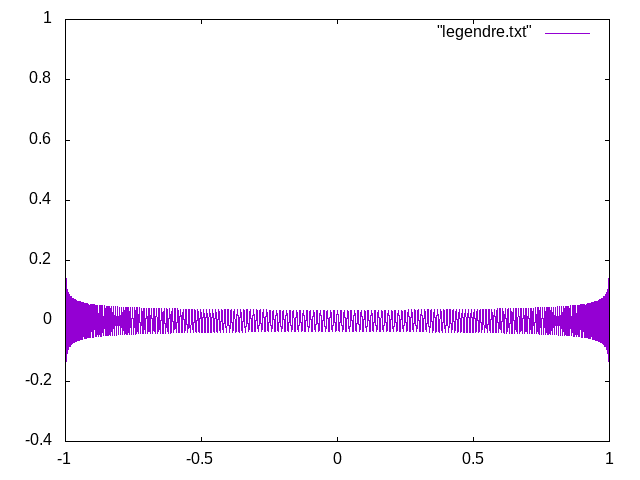
\includegraphics[width=0.8\linewidth]{../src/legendre}
\caption{勒让德函数$P_n(x)$。}
\label{fig:legendre1}
\end{figure}
\end{frame}

\begin{frame}{看图说话}
\begin{figure}
\centering
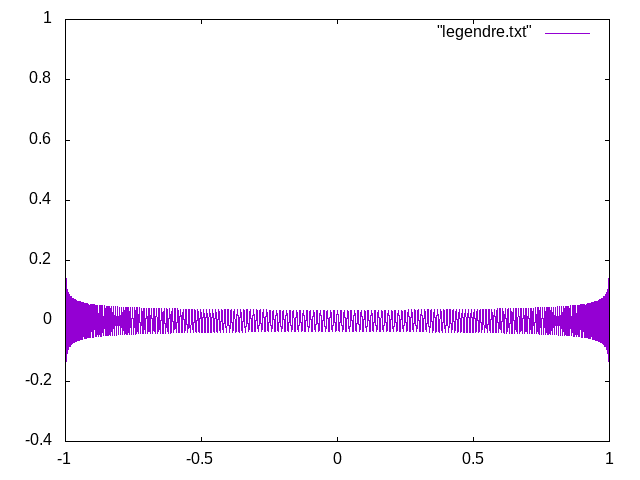
\includegraphics[width=0.5\linewidth]{../src/legendre}
\caption{勒让德函数$P_n(x)$。}
\label{fig:legendre2}
\end{figure}
仅归纳$P_0(x) \sim P_4(x)$,勒让德函数似乎有如下特点:
\begin{itemize}
\item [1] 函数值在$[-1,1]$之间。
\item [2] $P_0, P_2, P_4$为偶函数,$P_1,P_3$为奇函数。
\item [3] $P_n(x)$与$x$轴有$n$个交点,都在$(-1,1)$之间。
\end{itemize}

\end{frame}

\begin{frame}{求取勒让德函数:递推公式}
从母函数出发
\begin{equation}
G(x,z) = \frac{1}{ \sqrt{1-2xz+z^2} } = \sum^\infty_{n=0} P_n(x) z^n,
\end{equation}
等式两侧求偏导数得到
\begin{eqnarray}
\frac{\partial G}{\partial x} = z(1-2xz+z^2)^{-3/2} &=& \sum^\infty_{n=0} P'_n(x) z^n,
\label{eqn:legendre-partialx}
\\
\frac{\partial G}{\partial z} = (x-z)(1-2xz+z^2)^{-3/2} &=& \sum^\infty_{n=0} P_n(x) n z^{n-1}.
\label{eqn:legendre-partialz}
\end{eqnarray}

比较上面两式,可以得到
\begin{equation}
(x-z) \sum^\infty_{n=0} P'_n(x) z^n = z \sum^\infty_{n=0} P_n(x) n z^{n-1}.
\end{equation}

\end{frame}

\begin{frame}{递推公式}
两边取$z^n$项系数,得到
\begin{equation}
xP'_n(x) - P'_{n-1}(x) = nP_n(x).
\label{eqn:legendre-recursion1}
\end{equation}
另外,由(\ref{eqn:legendre-partialz}),有
\begin{equation}
(x-z) \sum^\infty_{n=0} P_n(x) z^n = (1-2xz+z^2) \sum^\infty_{n=0} P_n(x) n z^{n-1},
\end{equation}
取$z^n$项系数,即
\begin{equation}
xP_n(x) - P_{n-1}(x) = (n+1)P_{n+1}(x) - 2nxP_n(x) + (n-1)P_{n-1}(x),
\end{equation}
即
\begin{equation}
(n+1) P_{n+1}(x) - (2n+1)xP_n(x) + nP_{n-1}(x) = 0.
\label{eqn:legendre-recursion2}
\end{equation}
前面我们已经推得了$P_0(x)=1, P_1(x)=x$,结合上面的递推式,我们可以看出,$P_n(x)$就是一个{\bf $n$阶的多项式}。
\end{frame}

\begin{frame}{勒让德多项式}
\begin{equation}
(n+1) P_{n+1}(x) - (2n+1)xP_n(x) + nP_{n-1}(x) = 0.
\end{equation}
$P_0(x)=1, P_1(x)=x$,所以可以推得
\begin{eqnarray}
P_0(x) &=& 1, \\
P_1(x) &=& x, \\
P_2(x) &=& \frac{3}{2}x^2 - \frac{1}{2}, \\
P_3(x) &=& \frac{5}{2}x^3 - \frac{3}{2}x, \\
P_4(x) &=& \frac{35}{8}x^4 - \frac{15}{4}x^2 + \frac{3}{8}. \\
&\vdots& \nonumber
\end{eqnarray}
\end{frame}

\begin{frame}{递推式}
很容易由(\ref{eqn:legendre-recursion1},\ref{eqn:legendre-recursion2})得到另外两个递推式。
对(\ref{eqn:legendre-recursion2})求导数,得到
\begin{equation}
(n+1)P'_{n+1}(x) - (2n+1)P_n(x) - (2n+1)xP'_n(x) + nP'_{n-1}(x) = 0,
\end{equation}
而(\ref{eqn:legendre-recursion1})乘以$n$,有
\begin{equation}
n x P'_n(x) - nP'_{n-1}(x) = n^2 P_n(x),
\end{equation}
上面两式相加,得到
\begin{equation}
(n+1)P'_{n+1} - (n+1) xP'_n = (n+1)^2 P_n,
\end{equation}
即
\begin{equation}
P'_{n+1}(x) - xP'_{n}(x) = (n+1)P_n(x).
\label{eqn:legendre-recursion3}
\end{equation}
(\ref{eqn:legendre-recursion1},\ref{eqn:legendre-recursion3})相加,得到
\begin{equation}
P'_{n+1}(x) - P'_{n-1}(x) = (2n+1)P_n(x).
\label{eqn:legendre-recursion4}
\end{equation}

\end{frame}

\begin{frame}{递推式总结}

\begin{itemize}
\item [1] $xP'_n(x) - P'_{n-1}(x) = nP_n(x)$
\item [2] $(n+1) P_{n+1}(x) - (2n+1)xP_n(x) + nP_{n-1}(x) = 0$
\item [3] $P'_{n+1}(x) - xP'_{n}(x) = (n+1)P_n(x)$
\item [4] $P'_{n+1}(x) - P'_{n-1}(x) = (2n+1)P_n(x)$
\end{itemize}


\end{frame}

\begin{frame}{勒让德方程的导出}
递推式1与3如下, 
\begin{eqnarray}
xP'_n(x) - P'_{n-1}(x) &=& nP_n(x), \nonumber\\
P'_{n+1}(x) - xP'_{n}(x) &=& (n+1)P_n(x). \nonumber
\end{eqnarray}
第一个式子乘以$x$,第二个式子做$n+1 \rightarrow n$,得到
\begin{eqnarray}
x^2 P'_n(x) - x P'_{n-1}(x) &=& n x P_n(x), \nonumber\\
P'_{n}(x) - xP'_{n-1}(x) &=& n P_{n-1} (x). \nonumber
\end{eqnarray}
上两式相减,得到
\begin{equation}
(1-x^2)P'_n = nP_{n-1} - nxP_n,
\end{equation}
\end{frame}

\begin{frame}{勒让德方程}
\begin{equation}
(1-x^2)P'_n = nP_{n-1} - nxP_n,
\end{equation}
再求导数,得到
\begin{eqnarray}
(1-x^2)P''_n - 2xP'_n &=& nP'_{n-1} - nP_n - nxP'_n \nonumber\\
&=& -n P_n - n( xP'_n - P'_{n-1} ) \nonumber\\
&=& -nP_n - n^2 P_n = -n(n+1)P_n,
\end{eqnarray}
上面的推导使用了递推式1,
\begin{equation}
(1-x^2)P''_n - 2xP'_n + n(n+1)P_n = 0.
\end{equation}
换一句话说,$P_n$是以下微分方程的解
\begin{equation}
(1-x^2)y'' - 2x y' + n(n+1) y = 0.
\end{equation}
这就是勒让德方程。
\end{frame}

\begin{frame}{勒让德函数的正交性与归一性}
勒让德微分方程为:$[-1,1]$上,
\begin{equation}
(1-x^2) u'' - 2x u' + n(n+1) u = 0, -1 \leq x \leq 1.
\end{equation}
即$p_0 (x) = 1-x^2, p_1(x) = -2x, p_2(x) = 0, \omega(x) = 1, \lambda = n(n+1)$。
所以自然有,$n\neq m$时,勒让德函数$P_n, P_m$的正交性
\begin{equation}
\int^1_{-1} P_n(x) P_m(x) dx = 0.
\end{equation}

下面我们论证归一性,或者说,勒让德函数的模方,即
\begin{equation}
\int^1_{-1} P^2_n dx = \frac{2}{2n+1},
\end{equation}
\end{frame}

\begin{frame}{归一性}
证明:根据$(\ref{eqn:legendre-recursion2})$式,以及正交性,有
\begin{eqnarray}
\int^1_{-1} P^2_{n+1} dx &=& \frac{1}{n+1}\int^1_{-1} (2n+1) x P_n P_{n+1} dx 
\nonumber\\
&=& \frac{2n+1}{n+1} \int^1_{-1} x P_n P_{n+1} dx
\nonumber\\
&=& \frac{2n+1}{n+1} \int^1_{-1} P_n \frac{(n+2)P_{n+2} + (n+1)P_n}{2n+3} dx
\nonumber\\
&=& \frac{2n+1}{2n+3} \int^1_{-1} P^2_n dx,
\end{eqnarray}
由于$\int^1_{-1} P^2_0 dx = 2$,所以易得
\begin{equation}
\int^1_{-1} P^2_n dx = \frac{2n-1}{2n+1} \cdots \frac{1}{3} 2 = \frac{2}{2n+1}.
\end{equation}
\end{frame}

\begin{frame}{正交归一性}
综合正交性、归一性,得到
\begin{equation}
\int^1_{-1} P_n(x) P_m(x) dx =  \frac{2\delta_{nm}}{2n+1}.
\end{equation}
\end{frame}

\begin{frame}{完备性}
我们不加证明地给出完备性定理:若任意函数$f(x)$在区间$[-1,1]$上有连续的一阶导数、分段连续的二阶导数,则$f(x)$可以用$P_n(x)$做线性展开,
\begin{equation}
f(x) = \sum^\infty_{n=0} c_n P_n(x),
\end{equation}
右侧的级数形式一致收敛至$f(x)$。根据正交归一性,很容易写出
\begin{equation}
c_n = \frac{2n+1}{2} \int^1_{-1} f(x) P_n(x) dx, ~~~ n=0,1,2,\cdots
\end{equation}

\footnote{
思考:
\begin{itemize}
\item [1] 这个展开形式与傅里叶级数展开是多么的一致!像 $\left\{\cos nx, \sin nx \right\}$、$\left\{P_n(x)\right\}$这样的函数族,一定存在无穷多组,而任意“守规矩”的$f(x)$都可以用任意一族函数做线性展开!就像三维空间的3个基矢有无穷多种选取方式,函数空间的“基矢”选取也有无穷多种!
\item [2] 傅里叶级数通过形式变换+取极限,可以变为傅里叶积分,甚至傅里叶变换,勒让德函数展开,是否也能做类似的变形?
\end{itemize}
}

\end{frame}

\begin{frame}{多项式形式}
我们可以将母函数$G(x,z) = (1-2xz+z^2)^{-1/2}$进行级数展开,得到勒让德函数的多项式形式。
\begin{eqnarray}
G(x,z) = (1-2xz+z^2)^{-1/2} = \sum^\infty_{n=0} \frac{(2n)!}{2^{2n} (n!)^2} (2xz-z^2)^n,
\end{eqnarray}
这里使用了泰勒展开$(1-t)^{-1/2} = \sum^\infty_{n=0} \frac{(2n)!}{2^{2n} (n!)^2} t^{-1/2-n}$,上式进一步推导,得到
\begin{equation}
G(x,z) = \sum^\infty_{n=0} \frac{(2n)!}{2^{2n}(n!)^2} z^n \sum^n_{k=0} \frac{n!}{k! (n-k)!}(2x)^{n-k} (-z)^k,
\end{equation}
再做代换$n+k = m$,得到
\begin{equation}
G(x,z) = \sum^\infty_{m=0} z^m \sum^{[m/2]}_{k=0} \frac{(-1)^k (2m-2k)!}{2^m k! (m-k)! (m-2k)!} x^{m-2k}.
\end{equation}

\end{frame}

\begin{frame}{多项式形式}
所以总结下来,勒让德多项式为
\begin{equation}
P_n(x) = \sum^{[n/2]}_{k=0} \frac{(-1)^k (2n-2k)!}{2^n k! (n-k)! (n-2k)!} x^{n-2k}.
\end{equation}
\end{frame}

\begin{frame}{罗德里格斯公式(Rodrigues' Formula)}
因为$\frac{(2n-2k)!}{(n-2k)!}x^{n-2k} = \frac{d^n}{dx^n} x^{2n-2k}$,所以
\begin{eqnarray}
P_n(x) &=& \sum^{[n/2]}_{k=0} \frac{(-1)^k (2n-2k)!}{2^n k! (n-k)! (n-2k)!} x^{n-2k}
\nonumber\\
&=& \sum^{[n/2]}_{k=0} \frac{(-1)^k }{2^n k! (n-k)!} \frac{d^n}{dx^n} x^{2n-2k}
\end{eqnarray}
将求导数符号提前,得到
\begin{eqnarray}
P_n(x) &=& \frac{1}{2^n n!} \frac{d^n}{dx^n} \sum^{[n/2]}_{k=0} \frac{(-1)^k  n! }{ k! (n-k)!}  x^{2n-2k}
\nonumber\\
&=& \frac{1}{2^n n!} \frac{d^n}{dx^n} (x^2-1)^n
\end{eqnarray}
最后一行就是罗德里格斯公式。

\end{frame}

\begin{frame}{施拉夫利积分形式(Schlaefli Integral)}
罗德里格斯公式提供了便利,可以推导勒让德函数的围线积分形式。根据柯西积分公式
\begin{equation}
f^{(n)}(z) = \frac{n!}{2\pi i} \oint_C \frac{f(\zeta)}{(\zeta-z)^{n+1}}d\zeta,
\end{equation}
若取$f(z) = (z^2-1)^n$,则有
\begin{equation}
\frac{d^n}{dz^n} (z^2-1)^n = \frac{n!}{2\pi i} \oint_C \frac{(\zeta^2-1)^n}{(\zeta - z)^{n+1}} d \zeta,
\end{equation}
所以有
\begin{eqnarray}
P_n(x) &=& \frac{1}{2^n n!} \frac{d^n}{dx^n} (x^2-1)^n
= \frac{2^{-n}}{2\pi i} \oint_C \frac{(\zeta^2-1)^n}{(\zeta - x)^{n+1}} d \zeta.
\end{eqnarray}

\end{frame}

\begin{frame}{勒让德多项式 球函数}
\begin{itemize}
	\item 第一节:斯图姆-刘维尔理论
	\vspace{1cm}
	\item 第二节:勒让德多项式
	\vspace{1cm}
	\item {\color{blue}第三节:连带勒让德多项式}
	\vspace{1cm}
	\item 第四节:球函数、球形区域上的狄利克雷问题
\end{itemize}
\end{frame}

\begin{frame}{连带勒让德方程}
前面说明了,$P_n(x)$满足
\begin{equation}
(1-x^2)P''_n - 2xP'_n + n(n+1)P_n = 0,
\end{equation}
对整个方程求一次导数,得到
\begin{equation}
(1-x^2)P''' - 2 \cdot 2x P''_n + [n(n+1)-2]P'_n = 0,
\end{equation}
再次求导,得到
\begin{equation}
(1-x^2)P^{(2+2)}_n - 2(2+1)x P^{(2+1)}_n + [ n(n+1)- 2(2+1) ] P^{(2)}_n = 0,
\end{equation}
求$m$次导数,得到
\begin{equation}
(1-x^2)P^{(m+2)}_n - 2(m+1)x P^{(m+1)}_n + [ n(n+1)- m(m+1) ] P^{(m)}_n = 0,
\label{eqn:P^{(m+2)}_n}
\end{equation}
即$y = P^{(m)}_n(x)$满足常微分方程
\begin{equation}
(1-x^2)y'' - 2(m+1)xy' + [n(n+1)-m(m+1)] y = 0.
\end{equation}
\end{frame}

\begin{frame}{连带勒让德方程}
如果定义$z = (1-x^2)^{m/2} y = (1-x^2)^{m/2} P^{(m)}_n (x)$,则有$y = (1-x^2)^{-m/2}z$,
\begin{eqnarray}
y' &=& mx(1-x^2)^{-m/2-1} z + (1-x^2)^{-m/2} z', \nonumber\\
y'' &=& (1-x^2)^{-m/2} z'' + 2mx(1-x^2)^{-m/2-1}z'
\nonumber\\
&& + m(1-x^2)^{-m/2-2} z ( (m+2)x^2 + 1-x^2 )
\end{eqnarray}
得到
\begin{eqnarray}
(1-x^2) y'' &=& (1-x)^{-m/2+1} z'' + 2mx(1-x^2)^{-m/2}z'
\nonumber\\
&& + m(1-x^2)^{-m/2-1} z (1+(m+1)x^2), \nonumber\\
-2(m+1)xy' &=& -2m(m+1)x^2(1-x^2)^{-m/2-1} z \nonumber\\ &&-2(m+1)x(1-x^2)^{-m/2} z', \nonumber\\
\left[n(n+1)-m(m+1)\right] y &=& [n(n+1)-m(m+1)](1-x^2)^{-m/2}z. \nonumber
\end{eqnarray}
代入$(1-x^2)y-2(m+1)xy' + [n(n+1)-m(m+1)]y = 0$,
\end{frame}

\begin{frame}{连带勒让德方程}
整理以后得到
\begin{equation}
(1-x^2)z'' - 2x z' + [ n(n+1) - \frac{m^2}{1-x^2}] z = 0.
\end{equation}
这就是连带勒让德方程,定义连带勒让德多项式
\begin{equation}
P^m_n(x) = (1-x^2)^{m/2} P^{(m)}_n(x).
\end{equation}
$m=0$时退化为勒让德函数
\begin{equation}
P^0_n(x) = P_n(x).
\end{equation}
\end{frame}

\begin{frame}{连带勒让德函数的正交性}
连带勒让德微分方程为:$[-1,1]$上,
\begin{equation}
(1-x^2) u'' - 2x u' + [n(n+1) - \frac{m^2}{1-x^2}] u = 0, -1 \leq x \leq 1.
\end{equation}
即$p_0 (x) = 1-x^2, p_1(x) = -2x, p_2(x) = - \frac{m^2}{1-x^2}, \omega(x) = 1, \lambda = n(n+1)$。
所以自然有,$n\neq m$时,连带勒让德函数$P^m_n$的正交性:$k \neq n$时,
\begin{equation}
\int^1_{-1} P^m_k(x) P^m_n(x) dx = 0.
\end{equation}
\end{frame}

\begin{frame}{连带勒让德函数的模方}
下面我们求勒让德函数的模方,即$\int^1_{-1} [ P^m_n(x) ]^2 dx$,
有多种方法求这个值,这里我们使用教材上的思路
\begin{eqnarray}
\int^1_{-1} [ P^m_n(x) ]^2 dx &=& \int^1_{-1} (1-x^2)^m [ P^{(m)}_n ]^2 dx
\nonumber\\
&=& \int^1_{-1} (1-x^2)^m P^{(m)}_n \frac{d}{dx}P^{(m-1)}_n dx
\nonumber\\
&=& - \int^1_{-1} P^{(m-1)}_n \frac{d}{dx}[ (1-x^2)^m P^{(m)}_n ] dx.
\end{eqnarray}
在(\ref{eqn:P^{(m+2)}_n})中,用m-1代替m,得到
\begin{equation}
(1-x^2)P^{(m+1)}_n - 2mxP^{(m)}_n + [ n(n+1) - (m-1)m ] P^{(m-1)}_n = 0,
\end{equation}
两边同乘$(1-x^2)^{m-1}$,得到
\begin{eqnarray}
(1-x^2)^m P^{(m+1)}_n - 2mx(1-x^2)^{m-1} P^{(m)}_n 
\nonumber \\
+ [ n(n+1) - (m-1)m ](1-x^2)^{m-1} P^{(m-1)}_n = 0,
\end{eqnarray}
\end{frame}

\begin{frame}{连带勒让德函数的模方}
前两项正是
\begin{equation}
\frac{d}{dx} [ (1-x^2)^m P^{(m)}_n ],
\end{equation}
即
\begin{equation}
\frac{d}{dx} [ (1-x^2)^m P^{(m)}_n ] = - (n+m)(n-m+1)(1-x^2)^{m-1} P^{(m-1)}_n,
\end{equation}
所以有
\begin{eqnarray}
\int^1_{-1} [ P^m_n(x) ]^2 dx &=& - \int^1_{-1} P^{(m-1)}_n \frac{d}{dx}[ (1-x^2)^m P^{(m)}_n ] dx \nonumber\\
&=& (n+m)(n-m+1) \int^1_{-1} [P^{m-1}_n(x) ]^2 dx.
\end{eqnarray}
\end{frame}

\begin{frame}{连带勒让德函数正交归一性}
根据上面的递推式,得到
\begin{eqnarray}
&& \int^1_{-1} [ P^m_n(x) ]^2 dx \nonumber\\
&=& (n+m)(n+m-1) \cdots (n+1) (n-m+1)(n-m) \cdots n \nonumber\\
&& \times \int^1_{-1} [ P_n(x) ]^2 dx
\nonumber\\
&=& \frac{(n+m)!}{(n-m)!}\frac{2}{2n+1}.
\end{eqnarray}

总结正交性、归一性,得到
\begin{equation}
\int^1_{-1} P^m_n(x) P^m_k(x) dx = \frac{(n+m)!}{(n-m)!}\frac{2 \delta_{kn}}{2n+1}
\end{equation}

\end{frame}

\begin{frame}{勒让德多项式 球函数}
\begin{itemize}
	\item 第一节:斯图姆-刘维尔理论
	\vspace{1cm}
	\item 第二节:勒让德多项式
	\vspace{1cm}
	\item 第三节:连带勒让德多项式
	\vspace{1cm}
	\item {\color{blue}第四节:球函数、球形区域上的狄利克雷问题}
\end{itemize}
\end{frame}

\begin{frame}{球函数的导出}
在静电场问题、热稳态温度分布、量子力学问题中,都会出现拉普拉斯算子
\begin{equation}
\Delta = \nabla^2,
\end{equation}
其中$\vec{\nabla} = \vec{e}_x \partial_x + \vec{e}_y \partial_y + \vec{e}_z \partial_z$是梯度算符。
在球坐标系下,梯度算符可写作
\begin{equation}
\vec{\nabla} = \vec{e}_r \partial_r + \vec{e}_\theta \frac{1}{r}\partial_\theta + \vec{e}_\phi \frac{1}{r\sin \theta} \partial_\phi,
\end{equation}
三个基矢$\vec{e}_r, \vec{e}_\theta, \vec{e}_\phi$对$r,\theta,\phi$的偏导数为
\begin{eqnarray}
\begin{aligned}
& \partial_r \vec{e}_r = 0,~~ & \partial_r \vec{e}_\theta = 0,~~ & \partial_r \vec{e}_\phi = 0, \\
& \partial_\theta \vec{e}_r = \vec{e}_\theta,~~ & \partial_\theta \vec{e}_\theta = - \vec{e}_r,~~ & \partial_\theta \vec{e}_\phi = 0, \\
& \partial_\phi \vec{e}_r = \sin \theta \vec{e}_\phi, ~~
& \partial_\phi \vec{e}_\theta = \cos \theta \vec{e}_\phi, ~~
& \partial_\phi \vec{e}_\phi = - ( \vec{e}_r - \cos \theta \vec{e}_z )
\end{aligned}
\end{eqnarray}
利用这些偏导数,可以计算得到
\begin{equation}
\nabla^2 = \vec{\nabla} \cdot \vec{\nabla}
= \partial_r^2 + \frac{2}{r} \partial_r + \frac{1}{r^2} \partial_\theta^2 + \frac{1}{r^2} \frac{\cos \theta}{\sin \theta} \partial_\theta + \frac{1}{r^2 \sin^2 \theta} \partial_\phi^2.
\end{equation}
\end{frame}

\begin{frame}{球函数的导出}
球坐标下的拉普拉斯方程为
\begin{equation}
\nabla^2 u = 0,
\end{equation}
将$\nabla^2$在球坐标下的表达式代入,并做分离变量法$u = R(r) Y(\theta, \phi)$,得到
\begin{equation}
\frac{r^2}{R}( \frac{d^2}{dr^2}R + \frac{2}{r}\frac{dR}{dr} ) 
= - \frac{1}{Y}( \partial_\theta^2 Y + \cot \partial_\theta Y + \frac{1}{\sin^2 \theta} \partial_\phi^2 Y ) = \lambda,
\end{equation}
即分离出两个微分方程
\begin{eqnarray}
&& r^2 \frac{d^2}{dr^2}R + 2r \frac{dR}{dr} - \lambda R = 0, \\
&& \partial_\theta^2 Y + \cot \theta \partial_\theta Y + \frac{1}{\sin^2 \theta} \partial_\phi^2 Y + \lambda Y = 0.
\end{eqnarray}
此处的$Y(\theta, \phi)$即定义为球函数。
\end{frame}

\begin{frame}{球函数}
进一步分解球函数,记 $Y(\theta, \phi) = \Theta(\theta) \Phi(\phi)$,带入球函数的微分方程,得到
\begin{equation}
\frac{\sin^2 \theta}{\Theta} ( \frac{d^2}{d \theta^2} \Theta + \cot \theta \frac{d}{d \theta} \Theta )
+ \frac{1}{\Phi} \frac{d^2}{d \phi^2}\Phi + \lambda \sin^2 \theta = 0.
\end{equation}
若取$x = \cos \theta, \theta \in [0, \pi]$,则有
\begin{eqnarray}
\frac{d}{d\theta} &=& \frac{dx}{d \theta} \frac{d}{dx} = - \sin \theta \frac{d}{dx} = - \sqrt{1-x^2}\frac{d}{dx}, \\
\frac{\cos \theta}{\sin \theta} \frac{d}{d \theta} &=& - \cos \theta \frac{d}{dx} = - x \frac{d}{dx}, \\
\frac{d^2}{d \theta^2} &=& - \sin \theta \frac{d}{dx} ( - \sin \theta \frac{d}{dx}) = - \sqrt{1-x^2}\frac{d}{dx}( - \sqrt{1-x^2} \frac{d}{dx})
\\
&=& \sqrt{1-x^2}( \sqrt{1-x^2}\frac{d^2}{dx^2} - \frac{x}{\sqrt{1-x^2}}\frac{d}{dx} ) = (1-x^2) \frac{d^2}{dx^2} - x \frac{d}{dx}. \nonumber
\end{eqnarray}
\end{frame}

\begin{frame}{球函数}
所以$\Theta$满足的方程为
\begin{equation}
(1-x^2)^2 \frac{d^2}{dx^2}\Theta - (1-x^2) 2x \frac{d}{dx}\Theta + \lambda(1-x^2)\Theta = m^2\Theta,
\end{equation}
两边同除$(1-x^2)$,得到
\begin{equation}
(1-x^2) \frac{d^2}{dx^2}\Theta - 2x \frac{d}{dx}\Theta + (\lambda - \frac{m^2}{1-x^2} ) \Theta = 0.
\end{equation}
这正是连带勒让德方程。
总结下来,$u(r,\theta,\phi) = R(r) \Theta(\theta) \Phi(\phi)$,其中$R, \Theta, \Phi$分别满足
\begin{eqnarray}
&& r^2 \frac{d^2 R}{dr^2} + 2r \frac{dR}{dr} - \lambda R = 0, \\
&& (1-x^2) \frac{d^2}{dx^2}\Theta - 2x \frac{d}{dx}\Theta + (\lambda - \frac{m^2}{1-x^2} ) \Theta = 0, x = \cos \theta, \\
&& \frac{d^2}{d\phi^2}\Phi = - m^2 \Phi,
\end{eqnarray}
\end{frame}

\begin{frame}{球函数}
相应的$R, \Theta, \Phi$的解为
\begin{eqnarray}
&& R_n (r) = r^n, n=0,1,2,\cdots \\
&& \Phi_m (\phi) = \alpha_m \cos m \phi + \beta_m \sin m \phi, m = 0,1,2,\cdots \\
&& \Theta^m_n(\theta) = \gamma_n P^m_n (\cos \theta), ~~ m,n = 0,1,2,\cdots, m\leq n.
\end{eqnarray}
所以每个$n,m$对应的$u(r,\theta,\phi)$特解为
\begin{equation}
u^m_n(r,\theta, \phi) = R_n \Phi_m \Theta^m_n = r^n( a^m_n \cos m\phi + b^m_n \sin m \phi) P^m_n(\cos \theta),
\end{equation}
其中$a^m_n = \gamma_n \alpha_m, b^m_n = \gamma_n \beta_m$都是任意常数。
通解为
\begin{equation}
u(r,\theta, \phi) = \sum_{0\leq m \leq n \leq \infty} u^m_n(r, \theta, \phi).
\end{equation}
\end{frame}

\begin{frame}{球函数}
若有边界条件
\begin{equation}
u(r=l, \theta, \phi) = f(\theta, \phi),
\end{equation}
则将通解带入,得到
\begin{equation}
f(\theta, \phi) = \sum^\infty_{n=0} l^n [ \sum^n_{m=0} (a^m_n \cos m\phi + b^m_n \sin m \phi) P^m_n(\cos \theta) ].
\end{equation}
因为${1,\cos\phi, \cos 2 \phi, \cdots, \sin \phi, \sin 2 \phi, \cdots}$在$[0,2\pi]$是构成正交函数系,$P^m_m, P^m_{m+1}, \cdots$在$[-1,1]$上构成正交函数系,所以可以得到
\begin{eqnarray}
\footnotesize
a^0_n &=& \frac{2n+1}{4\pi l^n} \int^{2\pi}_0 \int^\pi_0 f(\theta, \phi) P_n(\cos \theta) \sin \theta d\theta d \phi, \\
a^m_n &=& \frac{(2n+1)(n-m)!}{2\pi l^n (n+m)!} \int^{2\pi}_0 \int^\pi_0 f(\theta, \phi) P^m_n(\cos \theta) \cos m\phi \sin \theta d\theta d \phi, \nonumber
\\
\\
b^m_n &=& \frac{(2n+1)(n-m)!}{2\pi l^n (n+m)!} \int^{2\pi}_0 \int^\pi_0 f(\theta, \phi) P^m_n(\cos \theta) \sin m\phi \sin \theta d\theta d \phi. 
\nonumber\\
\end{eqnarray}
\end{frame}

\begin{frame}{课后作业}
\kong[1]
课后习题 3, 4, 5, 6, 10
\end{frame}

\end{document}